\documentclass{standalone}
\usepackage{tikz}
\usetikzlibrary{patterns, positioning}


\begin{document}
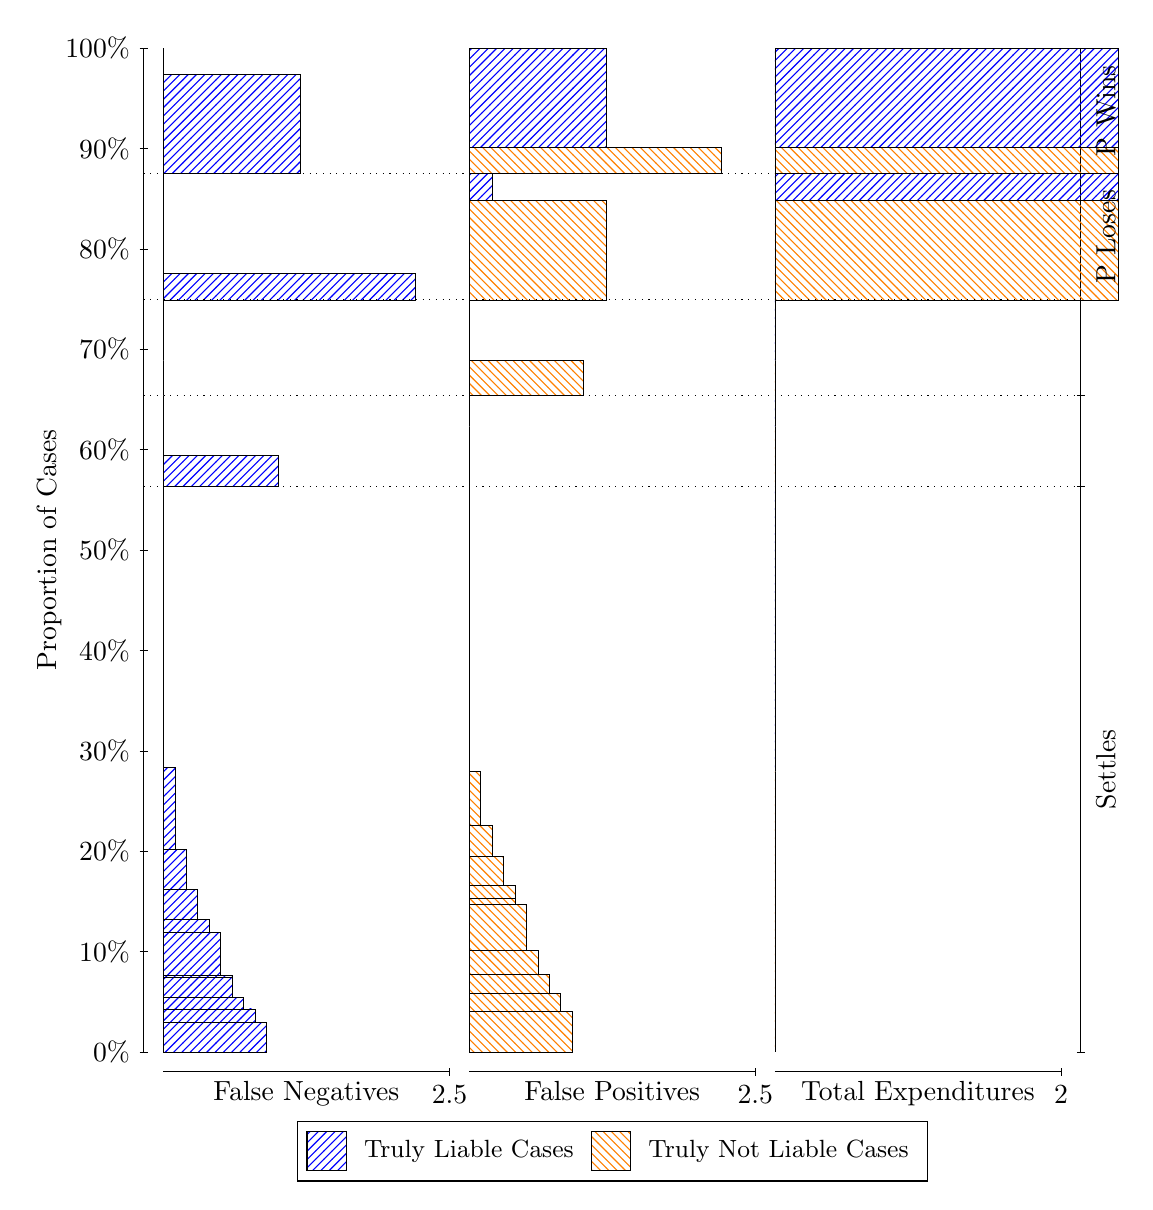
\begin{tikzpicture}
\draw[black, very thin] (1.5,1.75) -- (1.5,14.5);
\node[rotate=90, text=black, anchor=center] at (0.3, 8.125) {Proportion of Cases};
\draw[black, very thin] (1.45,1.75) -- (1.55,1.75);
\node[text=black, anchor=east] at (1.45, 1.75) {0\%};
\draw[black, very thin] (1.45,3.025) -- (1.55,3.025);
\node[text=black, anchor=east] at (1.45, 3.025) {10\%};
\draw[black, very thin] (1.45,4.3) -- (1.55,4.3);
\node[text=black, anchor=east] at (1.45, 4.3) {20\%};
\draw[black, very thin] (1.45,5.575) -- (1.55,5.575);
\node[text=black, anchor=east] at (1.45, 5.575) {30\%};
\draw[black, very thin] (1.45,6.85) -- (1.55,6.85);
\node[text=black, anchor=east] at (1.45, 6.85) {40\%};
\draw[black, very thin] (1.45,8.125) -- (1.55,8.125);
\node[text=black, anchor=east] at (1.45, 8.125) {50\%};
\draw[black, very thin] (1.45,9.4) -- (1.55,9.4);
\node[text=black, anchor=east] at (1.45, 9.4) {60\%};
\draw[black, very thin] (1.45,10.675) -- (1.55,10.675);
\node[text=black, anchor=east] at (1.45, 10.675) {70\%};
\draw[black, very thin] (1.45,11.95) -- (1.55,11.95);
\node[text=black, anchor=east] at (1.45, 11.95) {80\%};
\draw[black, very thin] (1.45,13.225) -- (1.55,13.225);
\node[text=black, anchor=east] at (1.45, 13.225) {90\%};
\draw[black, very thin] (1.45,14.5) -- (1.55,14.5);
\node[text=black, anchor=east] at (1.45, 14.5) {100\%};

\draw[black, very thin] (13.4,1.75) -- (13.4,14.5);
\draw[black, very thin] (13.35,1.75) -- (13.45,1.75);
\node[anchor=west] at (13.35, 1.75) {};
\draw[black, very thin] (13.35,8.9309) -- (13.45,8.9309);
\node[anchor=west] at (13.35, 8.9309) {};
\draw[black, very thin] (13.35,10.085) -- (13.45,10.085);
\node[anchor=west] at (13.35, 10.085) {};
\draw[black, very thin] (13.35,11.302) -- (13.45,11.302);
\node[anchor=west] at (13.35, 11.302) {};
\draw[black, very thin] (13.35,12.906) -- (13.45,12.906);
\node[anchor=west] at (13.35, 12.906) {};
\draw[black, very thin] (13.35,14.5) -- (13.45,14.5);
\node[anchor=west] at (13.35, 14.5) {};

\draw[black, very thin, pattern color=blue, pattern=north east lines] (1.75,1.75) rectangle (3.058,2.1255);
\draw[black, very thin, pattern color=blue, pattern=north east lines] (1.75,2.1255) rectangle (2.9127,2.2983);
\draw[black, very thin, pattern color=blue, pattern=north east lines] (1.75,2.2983) rectangle (2.7673,2.4393);
\draw[black, very thin, pattern color=blue, pattern=north east lines] (1.75,2.4393) rectangle (2.622,2.7012);
\draw[black, very thin, pattern color=blue, pattern=north east lines] (1.75,2.7012) rectangle (2.622,2.7262);
\draw[black, very thin, pattern color=blue, pattern=north east lines] (1.75,2.7262) rectangle (2.4767,3.2723);
\draw[black, very thin, pattern color=blue, pattern=north east lines] (1.75,3.2723) rectangle (2.3313,3.4343);
\draw[black, very thin, pattern color=blue, pattern=north east lines] (1.75,3.4343) rectangle (2.186,3.8173);
\draw[black, very thin, pattern color=blue, pattern=north east lines] (1.75,3.8173) rectangle (2.0407,4.3237);
\draw[black, very thin, pattern color=blue, pattern=north east lines] (1.75,4.3237) rectangle (1.8953,5.3676);
\draw[black, very thin, pattern color=orange, pattern=north west lines] (1.75,5.3676) rectangle (1.75,8.9309);
\draw[black, very thin, pattern color=blue, pattern=north east lines] (1.75,8.9309) rectangle (3.2033,9.3258);
\draw[black, very thin, pattern color=orange, pattern=north west lines] (1.75,9.3258) rectangle (1.75,10.085);
\draw[black, very thin, pattern color=orange, pattern=north west lines] (1.75,10.085) rectangle (1.75,10.533);
\draw[black, very thin, pattern color=blue, pattern=north east lines] (1.75,10.533) rectangle (1.75,11.302);
\draw[black, very thin, pattern color=blue, pattern=north east lines] (1.75,11.302) rectangle (4.9473,11.639);
\draw[black, very thin, pattern color=orange, pattern=north west lines] (1.75,11.639) rectangle (1.75,12.906);
\draw[black, very thin, pattern color=blue, pattern=north east lines] (1.75,12.906) rectangle (3.494,14.163);
\draw[black, very thin, pattern color=orange, pattern=north west lines] (1.75,14.163) rectangle (1.75,14.5);
\draw[black, very thin, pattern color=orange, pattern=north west lines] (5.6333,1.75) rectangle (6.9413,2.2678);
\draw[black, very thin, pattern color=orange, pattern=north west lines] (5.6333,2.2678) rectangle (6.796,2.4893);
\draw[black, very thin, pattern color=orange, pattern=north west lines] (5.6333,2.4893) rectangle (6.6507,2.7365);
\draw[black, very thin, pattern color=orange, pattern=north west lines] (5.6333,2.7365) rectangle (6.5053,3.0437);
\draw[black, very thin, pattern color=orange, pattern=north west lines] (5.6333,3.0437) rectangle (6.36,3.6233);
\draw[black, very thin, pattern color=orange, pattern=north west lines] (5.6333,3.6233) rectangle (6.2147,3.7011);
\draw[black, very thin, pattern color=orange, pattern=north west lines] (5.6333,3.7011) rectangle (6.2147,3.8675);
\draw[black, very thin, pattern color=orange, pattern=north west lines] (5.6333,3.8675) rectangle (6.0693,4.2324);
\draw[black, very thin, pattern color=orange, pattern=north west lines] (5.6333,4.2324) rectangle (5.924,4.6228);
\draw[black, very thin, pattern color=orange, pattern=north west lines] (5.6333,4.6228) rectangle (5.7787,5.3134);
\draw[black, very thin, pattern color=blue, pattern=north east lines] (5.6333,5.3134) rectangle (5.6333,8.9309);
\draw[black, very thin, pattern color=orange, pattern=north west lines] (5.6333,8.9309) rectangle (5.6333,9.6904);
\draw[black, very thin, pattern color=blue, pattern=north east lines] (5.6333,9.6904) rectangle (5.6333,10.085);
\draw[black, very thin, pattern color=orange, pattern=north west lines] (5.6333,10.085) rectangle (7.0867,10.533);
\draw[black, very thin, pattern color=blue, pattern=north east lines] (5.6333,10.533) rectangle (5.6333,11.302);
\draw[black, very thin, pattern color=orange, pattern=north west lines] (5.6333,11.302) rectangle (7.3773,12.569);
\draw[black, very thin, pattern color=blue, pattern=north east lines] (5.6333,12.569) rectangle (5.924,12.906);
\draw[black, very thin, pattern color=orange, pattern=north west lines] (5.6333,12.906) rectangle (8.8307,13.243);
\draw[black, very thin, pattern color=blue, pattern=north east lines] (5.6333,13.243) rectangle (7.3773,14.5);
\draw[black, very thin, pattern color=orange, pattern=north west lines] (9.5167,1.75) rectangle (9.5167,5.3134);
\draw[black, very thin, pattern color=blue, pattern=north east lines] (9.5167,5.3134) rectangle (9.5167,8.9309);
\draw[black, very thin, pattern color=orange, pattern=north west lines] (9.5167,8.9309) rectangle (9.5167,9.6904);
\draw[black, very thin, pattern color=blue, pattern=north east lines] (9.5167,9.6904) rectangle (9.5167,10.085);
\draw[black, very thin, pattern color=orange, pattern=north west lines] (9.5167,10.085) rectangle (9.5167,10.533);
\draw[black, very thin, pattern color=blue, pattern=north east lines] (9.5167,10.533) rectangle (9.5167,11.302);
\draw[black, very thin, pattern color=orange, pattern=north west lines] (9.5167,11.302) rectangle (13.877,12.569);
\draw[black, very thin, pattern color=blue, pattern=north east lines] (9.5167,12.569) rectangle (13.877,12.906);
\draw[black, very thin, pattern color=orange, pattern=north west lines] (9.5167,12.906) rectangle (13.877,13.243);
\draw[black, very thin, pattern color=blue, pattern=north east lines] (9.5167,13.243) rectangle (13.877,14.5);
\draw[black, dotted] (1.5,8.9309) -- (13.4,8.9309);
\draw[black, dotted] (1.5,10.085) -- (13.4,10.085);
\draw[black, dotted] (1.5,11.302) -- (13.4,11.302);
\draw[black, dotted] (1.5,12.906) -- (13.4,12.906);
\draw[black, very thin] (1.75,1.5) -- (5.3833,1.5);
\node[text=black, anchor=north] at (3.5667, 1.5) {False Negatives};
\draw[black, very thin] (5.3833,1.45) -- (5.3833,1.55);
\node[text=black, anchor=north] at (5.3833, 1.45) {2.5};

\draw[black, very thin] (5.6333,1.5) -- (9.2667,1.5);
\node[text=black, anchor=north] at (7.45, 1.5) {False Positives};
\draw[black, very thin] (9.2667,1.45) -- (9.2667,1.55);
\node[text=black, anchor=north] at (9.2667, 1.45) {2.5};

\draw[black, very thin] (9.5167,1.5) -- (13.15,1.5);
\node[text=black, anchor=north] at (11.333, 1.5) {Total Expenditures};
\draw[black, very thin] (13.15,1.45) -- (13.15,1.55);
\node[text=black, anchor=north] at (13.15, 1.45) {2};

\node[text=black, centered, rotate=90] at (13.72, 5.3405) {Settles};


\node[text=black, centered, rotate=90] at (13.72, 12.104) {P Loses};
\node[text=black, centered, rotate=90] at (13.72, 13.703) {P Wins};

\draw (7.449999999999999,1.5) node[draw=none] (baseCoordinate) {};
\begin{scope}[align=center]
        \matrix[scale=0.5, draw=black, below=0.5cm of baseCoordinate, nodes={draw}, column sep=0.1cm]{
            \node[rectangle, draw, minimum width=0.5cm, minimum height=0.5cm, pattern color=blue, pattern=north east lines] {}; &
            \node[draw=none, font=\small, text=black] (B) {Truly Liable Cases}; &
            \node[rectangle, draw, minimum width=0.5cm, minimum height=0.5cm, pattern color=orange, pattern=north west lines] {}; &
            \node[draw=none, font=\small, text=black] (B) {Truly Not Liable Cases}; \\
            };
\end{scope}

\end{tikzpicture}
\end{document}